\begin{blocksection}
Mutative (\emph{destructive}) operations change the state of a list by adding,
removing, or otherwise modifying the list itself.

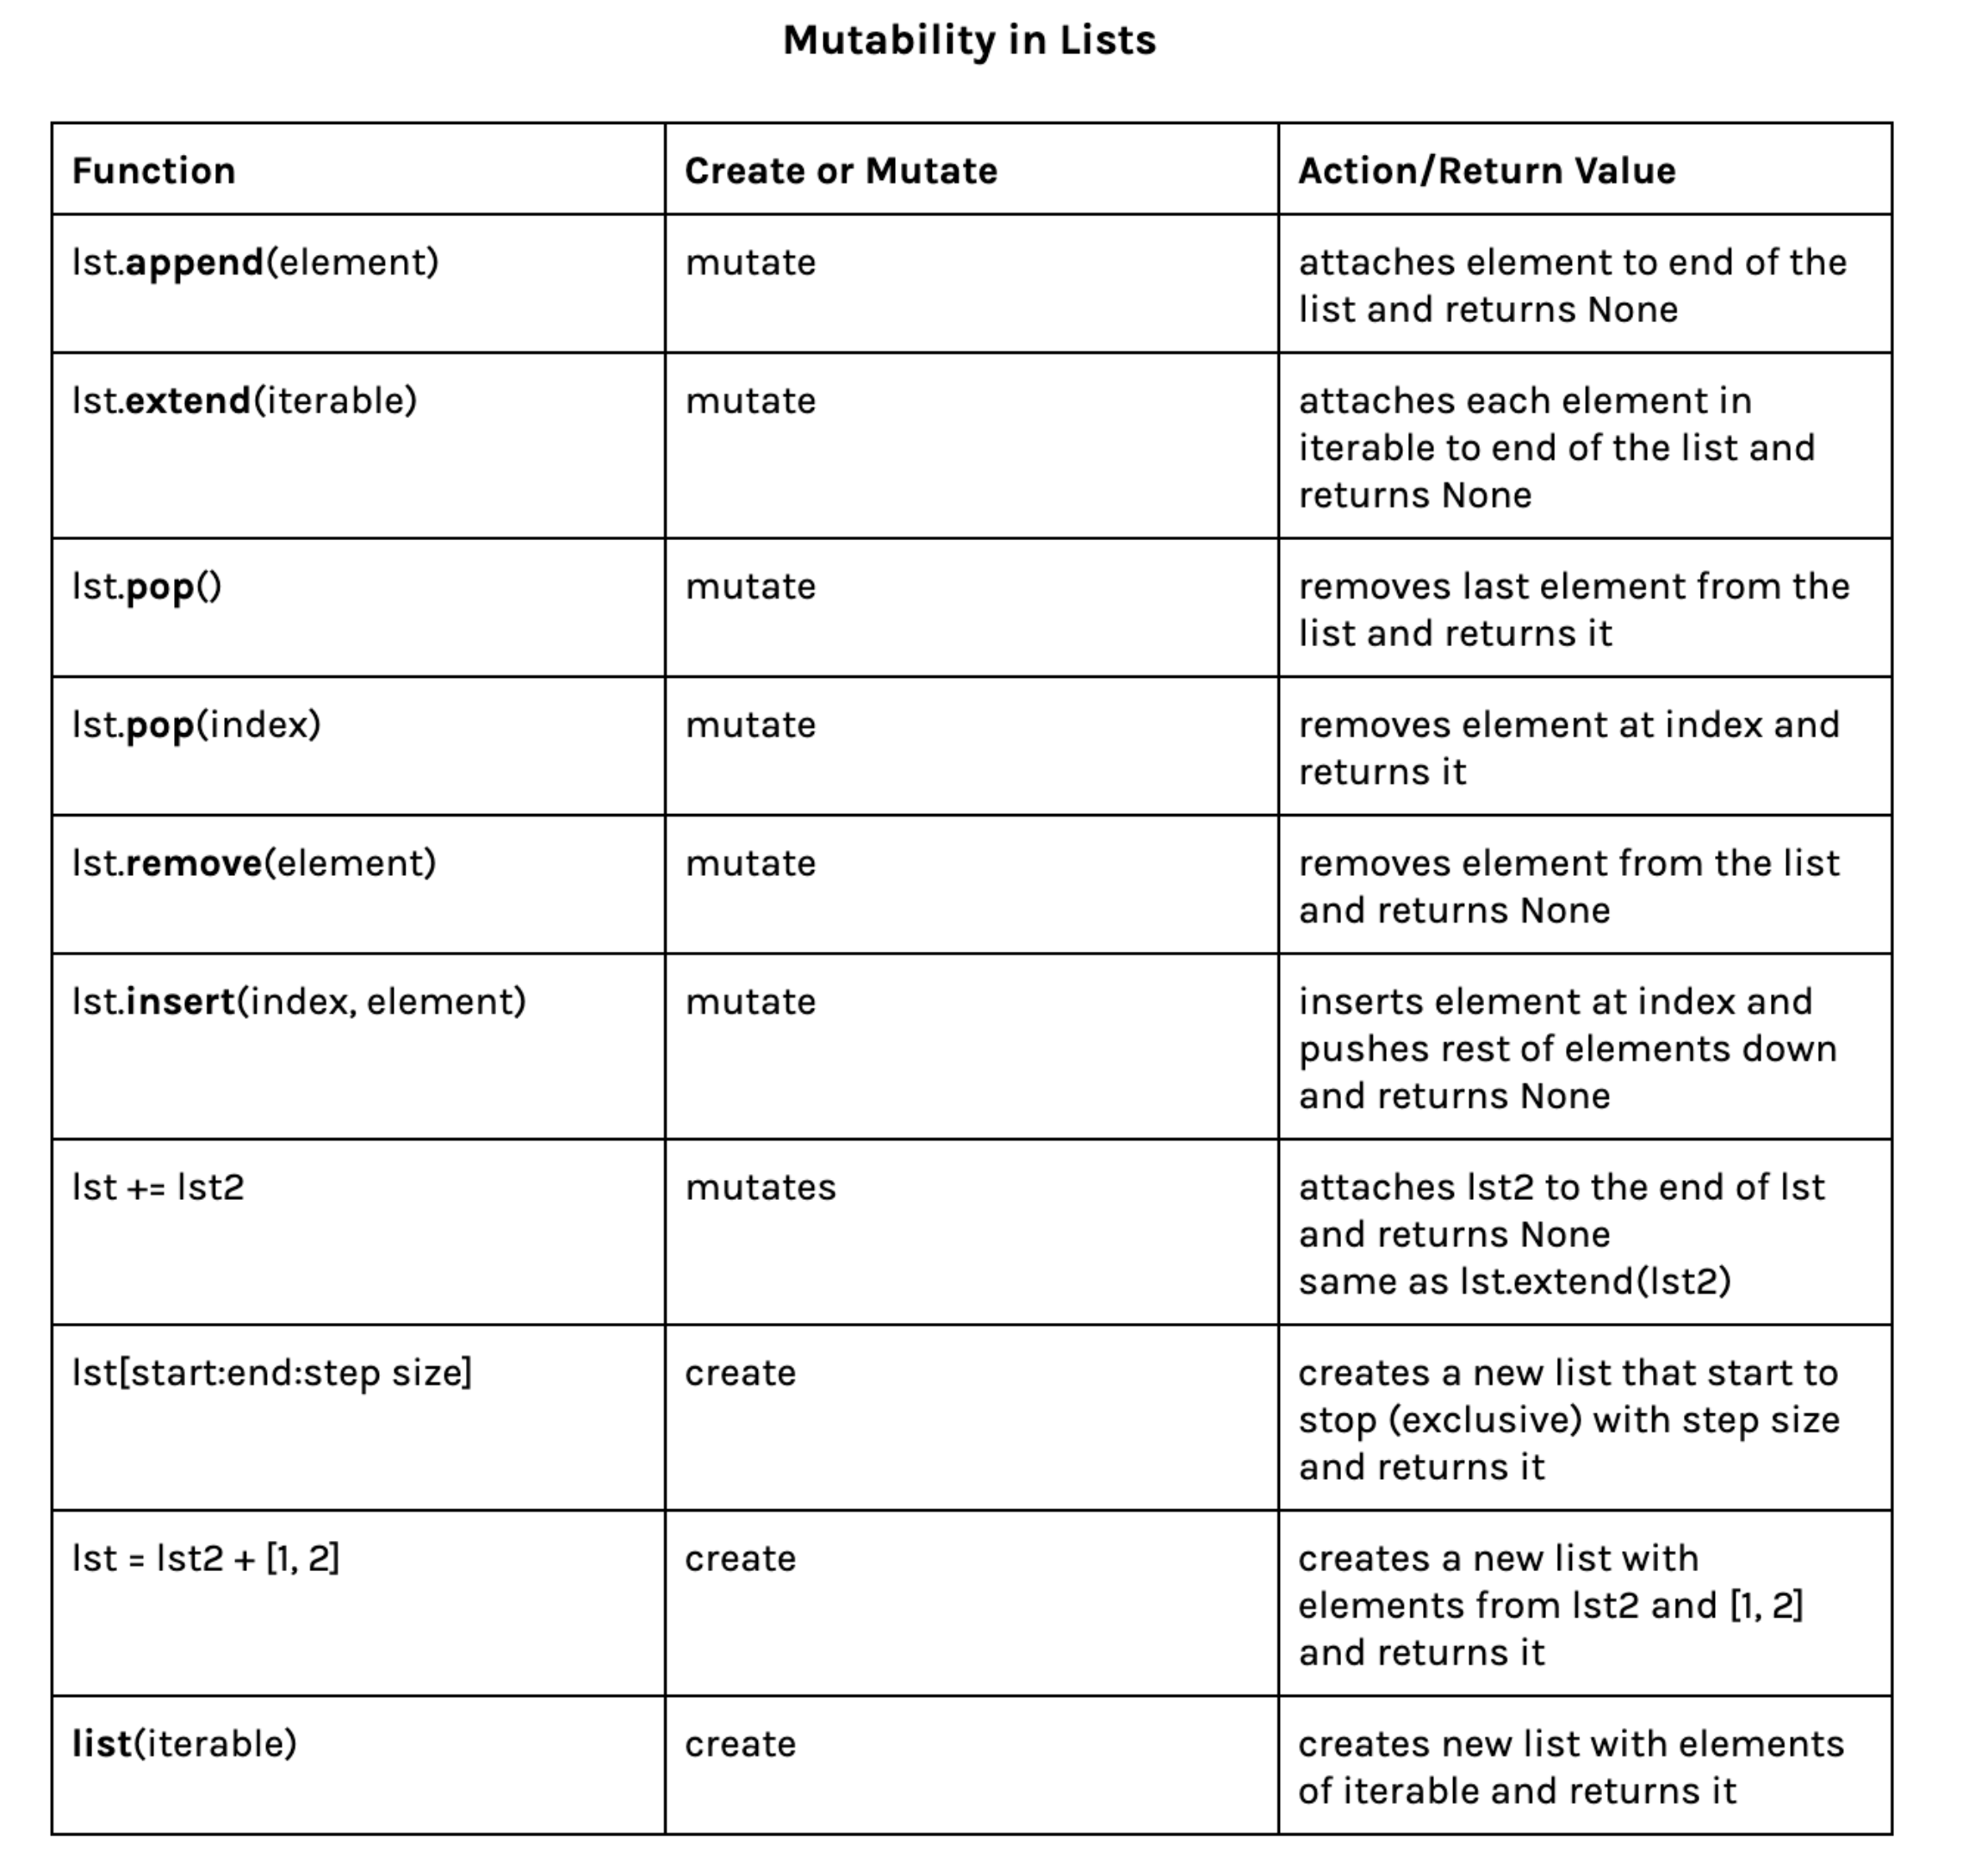
\includegraphics[width=.9\textwidth]{list-mutation.png}
\text{(credits: Mihira Patel)}

\begin{itemize}
\item \lstinline$lst.append(element)$
\item \lstinline$lst.extend(lst)$
\item \lstinline$lst.pop(index)$
\item \lstinline$lst += lst$ (\textbf{Note - this is different than:} \lstinline$lst = lst + lst$)
\item \lstinline$lst[i] = x$
\item \lstinline$lst[i:j] = lst$
\end{itemize}
\end{blocksection}

\vspace{\parskip}

\begin{blocksection}
Non-mutative (\emph{non-destructive}) operations do not change the original list but create a new list instead.

\begin{itemize}
\item \lstinline$lst + lst$
\item \lstinline$lst * n$
\item \lstinline$lst[i:j]$
\item \lstinline$list(lst)$
\end{itemize}
\end{blocksection}

\vspace{\parskip}
